\documentclass[11pt,a4paper]{article}
\usepackage[czech]{babel}
\usepackage[utf8]{inputenc}
\usepackage{times}
\usepackage{url}
\usepackage[textwidth=15.2cm,textheight=23cm]{geometry}
\usepackage{xcolor}

\usepackage{graphicx}

%\usepackage{fancyvrb}
%\DefineVerbatimEnvironment{verbatim}{Verbatim}{}

\usepackage[bf]{caption}

\usepackage[hyperindex,
  plainpages=false,
  pdftex,
  colorlinks,
  pdfborder={0 0 0},
  pdfpagelabels]{hyperref}

\pdfcompresslevel=9

\newcommand{\myincludegraphics}[4]{
  \begin{figure}[!h]
  \centering
  \includegraphics[#1]{#2}
  \caption{#3.} \label{#4}
  \end{figure}
}

% titulní stránka a obsah
\newcommand{\titlepageandcontents}{
  % credits for template go to: Martin Striz
\begin{titlepage}

\vspace*{1cm}

\begin{figure}
  \centering
  
\includegraphics[height=6cm]{images/fit.pdf}
\end{figure}

\vspace*{5mm}

\begin{center}
\begin{Large}
Projekt do předmětu GMU -- Grafické a multimediální procesory
\end{Large}
\end{center}

\vspace*{5mm}

\begin{center}
\begin{Huge}
Výpočet siluet pomocí GPU \\
\end{Huge}
\end{center}

\vspace*{1cm}

\begin{center}
\begin{Large}
\today
\end{Large}
\end{center}

\vfill

\begin{flushleft}
\begin{large}
\begin{tabular}{ll}

\bf Řešitelé:\hspace{3mm} & Zdeněk Biberle (\verb_xbiber00@stud.fit.vutbr.cz_) \\
& Vít Hodes (\verb_xhodes00@stud.fit.vutbr.cz_) \\
& Fakulta Informačních Technologií \\
& Vysoké Učení Technické v~Brně

\end{tabular}
\end{large}
\end{flushleft}

\end{titlepage}

% vim:set ft=tex expandtab enc=utf8:


  \pagestyle{plain}
  \pagenumbering{roman}
  \setcounter{page}{1}
  %\tableofcontents

  \newpage
  \pagestyle{plain}
  \pagenumbering{arabic}
  \setcounter{page}{1}
}

\def\uv#1{\iflanguage{english}{``#1''}%
                              {\quotedblbase #1\textquotedblleft}}%

% vim:set ft=tex expandtab enc=utf8:


\begin{document}
\titlepageandcontents

%---------------------------------------------------------------------------
\section{Zadání}

Implementace generovaní shadow volumes siluet pomocí compute shaderů a následné využití těchto siluet
pro tvorbu stínů pomocí z-fail algoritmu.

%---------------------------------------------------------------------------
\section{Použité technologie}

\section{Technologie potřebné pro běh}
\begin{itemize}
	\item Grafický akcelerátor s podporou OpenGL 4.3
		\begin{itemize}
			\item SSBO
			\item Image load/store
			\item Compute shadery
		\end{itemize}
	\item SDL2
	\item GLM
	\item glew
\end{itemize}

\section{Technologie použité pro tvorbu}
\begin{itemize}
	\item Blender
	\item Textový editor/vývojové prostředí vlastní volby
\end{itemize}

%---------------------------------------------------------------------------
\section{Použité zdroje}
	\begin{itemize}
		\item Stanford bunny
	\end{itemize}
%---------------------------------------------------------------------------
\section{Nejdůležitější dosažené výsledky}

\subsection {Generování stínového tělesa, jeho vykreslení a vizualizace}

\begin{figure}[h]
	\captionsetup{type=figure}
	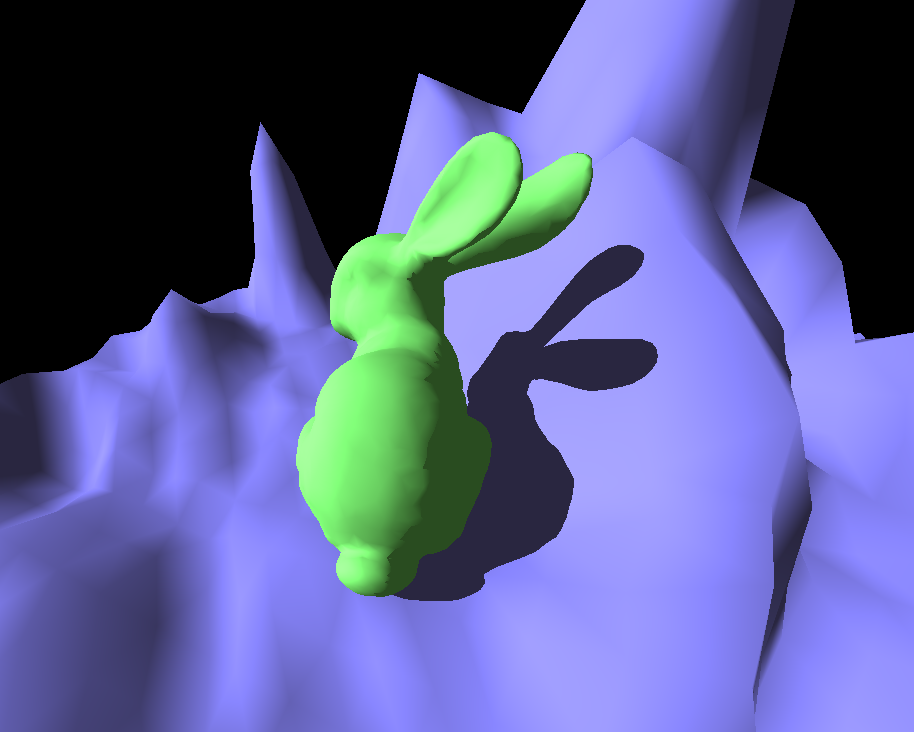
\includegraphics[width=\textwidth]{images/bunny.png}
	\captionof{figure}{Textura mraky.glsl}
\end{figure}

Funguje generování shadow volume na Nvidia kartách.

%---------------------------------------------------------------------------
\section{Ovládání vytvořeného programu}

\begin{itemize}
	\item Levé tlačítko myši - Společně s pohybem myši umožňuje změnu úhlu pohledu na scénu.
	\item Kolečko myši - Přiblížení a oddálení zobrazené scény.
	\item Klávesa R - Přepíná autonomní otáčení zobrazené scény.
	\item Klávesa T - Přepíná zobrazení vypočteného stínového tělesa.
	\item Klávesa C - Přepíná mezi CPU a GPU implementací výpočtu stínového tělesa.
\end{itemize}

%---------------------------------------------------------------------------
\section{Zvláštní použité znalosti}

Použití OpenGL compute shaderů se různě liší od použití OpenCL či CUDA. To vyžadovalo získání dodatečných informací o jejich využívání a o komunikaci s němi.
Využití image load/store v shaderech openGL pro vytvoření vlastního "stencil bufferu".

%---------------------------------------------------------------------------
\section{Rozdělení práce v týmu}

\paragraph{Zdeněk Biberle} Základ aplikace, compute shader pro výpočet stínového tělesa.
\paragraph{Vít Hodes} Vykreslení scény za použití stínového tělesa, nahrávání modelů.

%---------------------------------------------------------------------------
\section{Co bylo nejpracnější}

\paragraph{Zdeněk Biberle}

Značnou část času jsem strávil nad komunikací mezi aplikací a compute shaderů. Později jsem zjistil, že implementace SSBO na grafických kartách od AMD se v současnosti vyznačuje různými problémy a tudíž jsem řešil nevyřešitelné.

\paragraph{Vít Hodes} Přijít na to, jak impementovat celočíselný "stencil buffer" s obecným přístupem ze shaderů. Po prozkoumání několika slepých cest se dospělo k řešení pomocí iimage2D a atomického sčítání. Taky implementovat stíny nad shadow volume, který se mi na AMD kartě negeneruje správně se moc nedá.

%---------------------------------------------------------------------------
\section{Zkušenosti získané řešením projektu}

\paragraph{Zdeněk Biberle}
\begin{itemize}
	\item Compute shadery
	\item SSBO
\end{itemize}

\paragraph{Vít Hodes}
\begin{itemize}
	\item Framebuffer object, color/depth attachment
	\item v GLSL existují i shadow samplery a image samplery
	\item image load/store, atomické operace obecně v shaderech
	
\end{itemize}

%---------------------------------------------------------------------------
\section{Autoevaluace}

\paragraph{Technický návrh (70\%):} (analýza, dekompozice problému, volba
vhodných prostředků, $\ldots$) 


\paragraph{Programování (70\%):} (kvalita a čitelnost kódu, spolehlivost běhu,
obecnost řešení, znovupoužitelnost, $\ldots$)
Vzhledem ke kratšímu rozsahu se moc neuplatnuje zapouzdření ve vykreslovací části. Znovupoužitelnost
spíše znalostí než konkrétního kódu.

\paragraph{Vzhled vytvořeného řešení (40\%):} (uvěřitelnost zobrazení,
estetická kvalita, vhled GUI, $\ldots$)
Estetická kvalita nebyla cílem řešení.

\paragraph{Využití zdrojů (70\%):} (využití existujícího kódu a dat, využití
literatury, $\ldots$)
Bez dokumentací OpenGL API by tento projekt nevznikl.

\paragraph{Hospodaření s časem (50\%):} (rovnoměrné dotažení částí projektu,
míra spěchu, chybějící části řešení, $\ldots$)
Přiměřené. 

\paragraph{Spolupráce v týmu (80\%):} (komunikace, dodržování dohod, vzájemné
spolehnutí, rovnoměrnost, $\ldots$)
Komunikace dobrá.

\paragraph{Celkový dojem (70\%):} (pracnost, získané dovednosti, užitečnost,
volba zadání, cokoliv, $\ldots$)
Projekt byl zajímavý a potenciálně velmi užitečný. Škoda problémů s různými platformami(AMD x Nvidia).

%---------------------------------------------------------------------------
\section{Doporučení pro budoucí zadávání projektů}

Témata projektů byla dostatečně pestrá, ale příště by mohla být zadána dříve.

%---------------------------------------------------------------------------
\section{Různé}

Ještě něco by v dokumentaci mělo být? Napište to sem! Podle potřeby i založte
novou kapitolu.

\end{document}
% vim:set ft=tex expandtab enc=utf8:
